\section{Approfondissement technique sur la sécurité}
\paragraph{}
Cette section du rapport rassemble des points plus technique concernant Octopus Supervisor. Elle met en avant les points d'honneur fait sur la sécurité du logiciel.

\subsection{SSL}
\paragraph{}
Dès le lancement du projet, nous avions décidé que le client et le serveur échangerait des données chiffrées par SSL. 
Toutes les communications à travers des sockets utilisent le protocole SSL (Secure Socket Layer). Nous avons donc auto-signé un certificat pour le serveur.
Une authentification SSL est effectuée à chaque ouverture de socket entre les extrémités serveur et client.
\paragraph{}
Les échanges du serveur Web se font aussi avec le protocole SSL, nous avons donc une sécurisation des commandes de l'administrateur depuis l'interface Web.
Ceci nous permet d'assurer la confidentialité des données de bout en bout lors des communication entre des entités.

\subsection{Handshake}
\paragraph{}
Octopus Supervisor travaille avec un serveur et plusieurs clients. Afin de savoir avec qui l'on communique, il y a une phase d'authentification au début d'un échange entre deux entités.
Cette authentification est appelée "handshake", signifiant poignée de main. Elle commence par un message initiant la communication puis un acquittement. Ensuite il y a un échange d'ID pour identifier le Tentacle.
La dernière étape du Handshake est de vérifier la clé correspondant à l'ID qui a été générée lors de l'enregistrement du Tentacle sur le Brain.

\begin{figure}[!h]
	\centering
	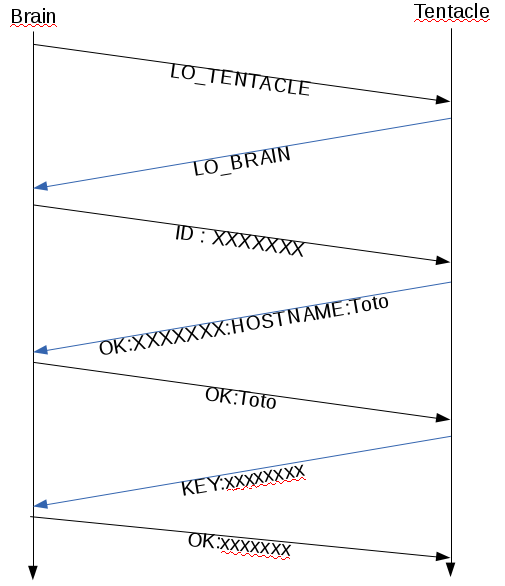
\includegraphics[scale=0.55]{img/handshake_register_btot.png}
        \caption{Handshake enregistrement}
\end{figure}

\paragraph{}
La Figure 5 représente l'initialisation de la communication entre le Brain et un Tentacle lors de l'enregistrement du dernier sur le Brain. Quand le Brain reçoit une adresse IP à ajouter à sa base de données, la communication suivante est effectuée.

\begin{figure}[!h]
	\centering
	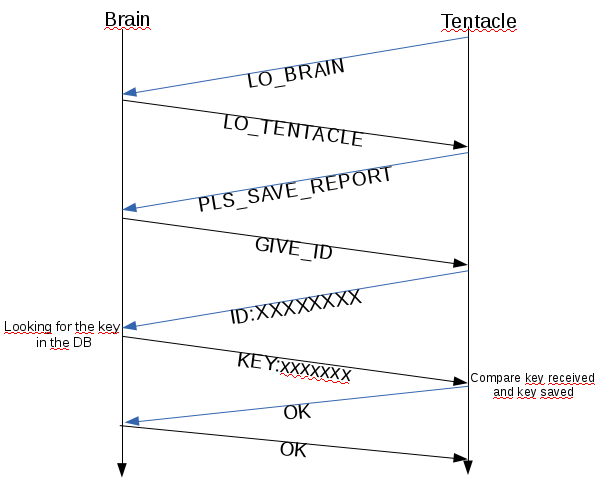
\includegraphics[scale=0.6]{img/handshake_commander_ttob.png}
	\caption{Handshake envoi résultat}
\end{figure}

\paragraph{}
La Figure 6 présente le handshake qui est fait lorsqu'un Tentacle contacte le Brain pour envoyer un résultat de script.
\paragraph{}

\subsection{Timeout web}
\paragraph{}
L'utilisation de Octopus Supervisor se fait grâce à une interface Web. Celle-ci nécessite une connexion avec un login et un mot de passe pour pouvoir identifier les administrateurs du logiciel.
Lorsqu'un utilisateur du logiciel se connecte à l'interface Web, une clé de session est créée et un timer est lancé. Si au bout de 300 secondes, l'utilisateur n'a pas interagi avec le WebServ, la clé de session ne sera plus valide et l'utilisateur sera automatiquement déconnecté.
Cela permet d'éviter une connexion permanente qui expose aux risques d'usurpation d'identité par session d'utilisateur.
